\section{Kolmogorov-Arnold Networks (KAN)}
The idea is to better approximate smooth functions with B-splines.

\subsection{B-Splines}
B-Splines are recursivly defined over a local area of knots(x coordinates)
Defined as \(B_{x-position,order}\).
\begin{figure}
    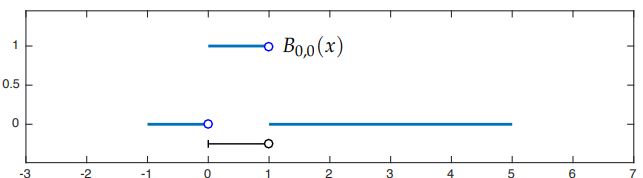
\includegraphics[width=0.5\columnwidth]{figures/KAN/BSplines1.png}
    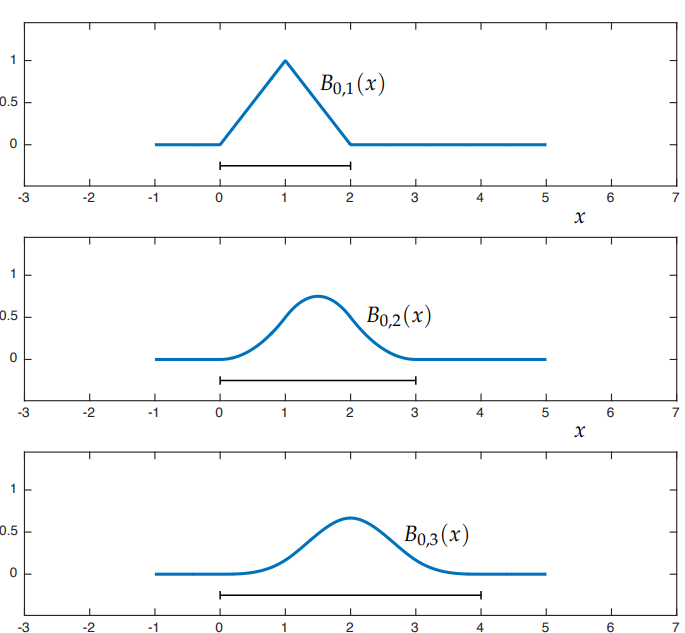
\includegraphics[width=0.5\columnwidth]{figures/KAN/BSplines2.png}
\end{figure}

\begin{figure}
    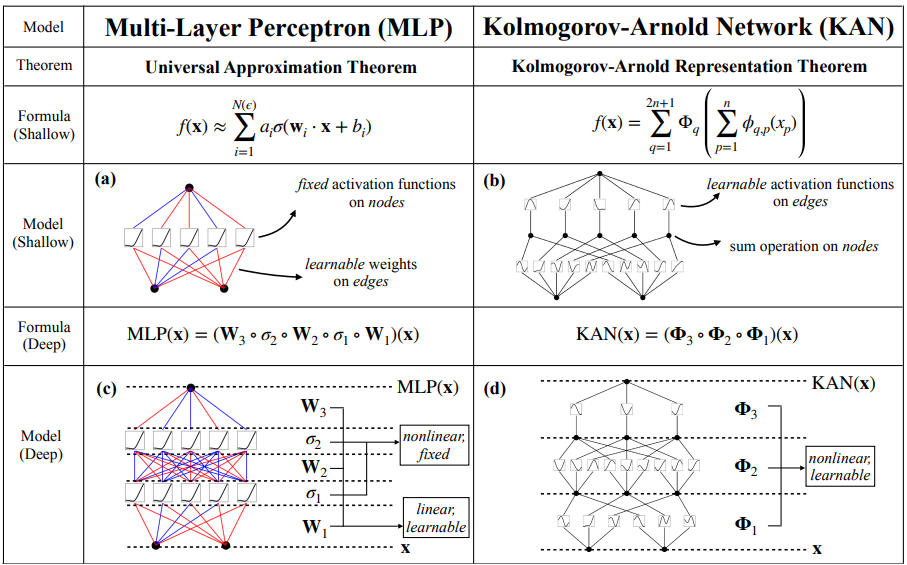
\includegraphics[width=\columnwidth]{figures/KAN/OverviewKANMLP.png}
\end{figure}
\begin{itemize}
    \item One main idea with the KANs is that they have better interpretability
    \item Aimed at math and physics applications
\end{itemize}
\subsection{Architecture}
\begin{itemize}
    \item Activation are on edges, not nodes, the nodes only do summation (no parameters)
    \item Non-linearity is applied on the edges before summing
\end{itemize}